\documentclass[../main2.tex]{subfiles}
\begin{document}
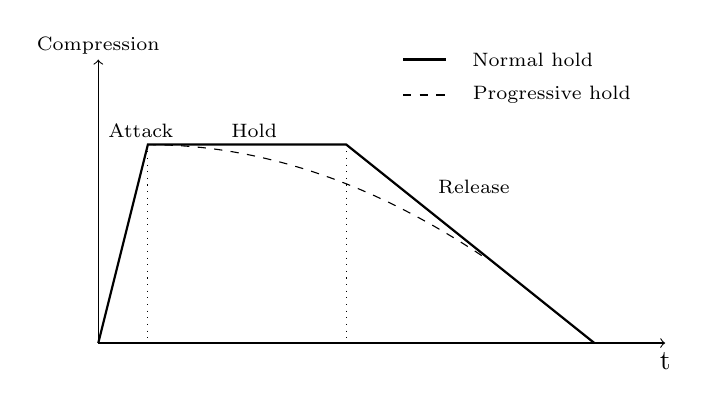
\begin{tikzpicture}[scale=0.9,baseline={(0,0)}]

%AXES
% horizontal axis
\draw[->] (0,0) -- (8,0) node[anchor=north] {t};
% vertical axis
\draw[->] (0,0) -- (0,4) node[anchor=north] {};
\draw(0, 4.2) node{{\scriptsize Compression}};

%GRAPH
%Integrator
\draw[thick] (0,0) -- (0.7,2.8) -- (1.8,2.8) -- (3.5,2.8) -- (7.0,0);
\draw[dashed,domain=0.7:5.5] plot (\x,{-0.070547*(-39.2-1.4*\x+(\x)^2))});
%Progressive hold
\draw[dotted] (0.7, 2.8) -- (0.7, 0);
\draw[dotted] (3.5, 2.8) -- (3.5, 0);

%LABELS
\draw(0.6, 3) node{{\scriptsize Attack}};
\draw(2.2,3) node{{\scriptsize Hold}};
\draw(5.3,2.2) node{{\scriptsize Release}};

%
\draw[thick] (4.3,4) -- (4.9,4);
\draw(6.13, 4) node{{\scriptsize Normal hold}};

\draw[dashed] (4.3,3.5) -- (4.9,3.5);
\draw(6.4, 3.5) node{{\scriptsize Progressive hold}};

\end{tikzpicture}
\end{document}
